\documentclass{beamer}

\usepackage{txfonts}
\usepackage{hyperref}
\usepackage{fancybox}
\usepackage{xfrac}
\usepackage{cancel}

\newcommand{\heart}{\ensuremath\heartsuit}

\usepackage{mathtools,amssymb}
\newcommand{\myarrow}{\scalebox{2}[2]{$\mathclap{\curvearrowleft}\mkern2.2mu
                                                 \mathclap{\curvearrowright}$}}

\DeclareMathOperator{\Bin}{\mathrm{Bin}}

\hypersetup{colorlinks=false,linkbordercolor=red,linkcolor=green,pdfborderstyle={/S/U/W 1}}

\addtobeamertemplate{navigation symbols}{}{ \hspace{1em}    \usebeamerfont{footline}%
    \insertframenumber / \inserttotalframenumber}

\geometry{papersize={15cm,15cm}}
\usepackage{lipsum}

\makeatletter
\newenvironment<>{contdproof}[1][\proofname]{%
    \par
    \def\insertproofname{#1\@addpunct{.}}%
    \usebeamertemplate{proof begin}#2}
  {\usebeamertemplate{proof end}}
\makeatother


\setbeamertemplate{theorems}[numbered]

\newtheorem*{nonumdefinition}{Definition}
\newtheorem*{nonumproblem}{Problem}
\newtheorem*{nonumcorollary}{Corollary}
\newtheorem*{nonumproof}{Proof}
\newtheorem*{nonumtheorem}{Theorem}
\newtheorem*{nonumremark}{Remark}
\newtheorem*{answer}{Answer}
\newtheorem*{nonumremarks}{Remarks}
\newtheorem*{nonumexamples}{Examples}
\newtheorem*{nonumsolution}{Solution}
\newtheorem*{nonumexample}{Example}
\newtheorem*{nonumproposition}{Proposition}
\newtheorem{proposition}[theorem]{Proposition}

\usepackage{tikz}
\newcommand*\mycirc[1]{%
  \tikz[baseline=(C.base)]\node[draw,circle,inner sep=.7pt](C) {#1};\:
}

\newcommand\myheading[1]{%
  \par\bigskip
  {\color{blue}{\large #1}}\par\smallskip}

%\usetheme{Warsaw}
%\usetheme{Berkeley} %sample 1

\usetheme{Berlin} % sample 2
%\usetheme{AnnArbor} % sample 3

\let\otp\titlepage
\renewcommand{\titlepage}{\otp\addtocounter{framenumber}{-1}}

\title{Lecture 13 : The Exponential Distribution}
\author{}
\date{}

\begin{document}
\begin{frame}[plain]
\titlepage
\end{frame}

\begin{frame}
\begin{nonumdefinition}
A continuous random variable $X$ is said to have exponential distribution with parameter $\lambda$.

If the $pdf$ of $X$ is (with $\lambda>0$)
\begin{equation*}
f(x)=
\left\{
\begin{array}{ll}
\lambda e^{-\alpha x}, & x>0\\
0, & \text{otherwise}
\end{array}
\right.\tag{*}\label{eq-*}
\end{equation*}
\end{nonumdefinition}

\begin{nonumremarks}
Very often the independent variable will be time $t$ rather than $x$. The exponential distribution is the special case of the gamma distribution with $\alpha=1$ and $\beta=\dfrac{1}{\alpha}$. We will see that $X$ \underline{$\beta$ closely tied to the Poisson process}, that is why $\lambda$ is used above.
\end{nonumremarks}
\end{frame}

\begin{frame}
Here is the graph of $f$

\smallskip
\centerline{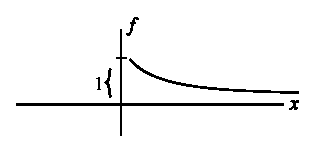
\includegraphics{figure/fig1.eps}}

\begin{nonumproposition}[(cdf) (Prove this)]
If $X$ has exponential distribution then
$$
F(x) =P(X\leq x)=1-e^{-\alpha x}
$$
\end{nonumproposition}

\begin{nonumcorollary}[Prove this]
If $X$ has exponential distribution
$$
P(X>x)=e^{-\lambda x}
$$
This is a very useful formula.
\end{nonumcorollary}
\end{frame}

\begin{frame}
\begin{nonumproposition}
If $X$ has exponential distribution
\begin{itemize}
\item[(i)] $E(X)=\dfrac{1}{\lambda}$

\item[(ii)] $V(X)=\dfrac{1}{\lambda^{2}}$
\end{itemize}
\end{nonumproposition}

\myheading{The Physical Meaning of the Exponential Distribution}

Recall (Lecture 8) that the binomial process (having a a child, flipping a coin) gave rise to two (actually infinitely many) more distributions
\begin{enumerate}
\item 
\begin{tabbing}
$X$ \== the geometric distribution\\
    \>= the waiting time for the first girl
\end{tabbing}
\end{enumerate}
\end{frame}

\begin{frame}
\begin{tabbing}
and\quad $X_{r}$ \== the negative binomial\\
                    \>= the waiting time for the $r$-th girl
\end{tabbing}

\begin{nonumremark}
Here time was discrete. Also $X_{r}$ was the \underline{number of boys} before the $r$-th girl so the waiting time was actually  $Y_{r}=X_{r}+r-1$.
\end{nonumremark}

Now we will see the same thing happens with a Poisson process. Now time is continuous, as I warned you. I will switch from $x$ to $t$ in \eqref{eq-*}.
\end{frame}

\begin{frame}
So suppose we have a trap to catch some species of animal. We run it forever starting at time $t=0$, so $0\leq t<\infty$.

\myheading{The Counting Random Variable}

Now fix a time period $t$. So we have a ``counting random variable $X_{t}$''.

$X_{t}=\sharp$ of animals caught in the trap in time $t$.

We will choose the model $X_{t}\sim P(\lambda t)=$ Poisson with parameter $\lambda t$.

{\large\bf Z} We are using $\lambda$ instead of $\alpha$ in the Poisson process

N.B. $P(X_{t}=0)=e^{-\lambda t}(\sharp)$
\end{frame}

\begin{frame}
\begin{nonumremark}
The analogue from before was

$X_{n}=\sharp$ of girls in the first $n$ children

(so we have a discrete ``time period'', the binomial random variable was the \underline{counting random variable.})

Now we want to consider the analogue of the ``waiting time'' random variables, the geometric and negative binomials for the binomial process.

Let $Y$ = the time when the first animal is caught.
\end{nonumremark}
\end{frame}

\begin{frame}
The proof of the following theorem involves such a beautiful simple idea I am going to give it.

\begin{nonumtheorem}
$Y$ has exponential distribution with parameter $\alpha$.
\end{nonumtheorem}

\begin{nonumproof}
We will compute $P(Y>t)$ and show $P(Y>t)=e^{-\lambda t}$ 
\begin{align*}
(\text{so~ } F(t) &= P(Y\leq t)=1-e^{-\lambda t}\\
\text{and~ } f(t) &= F'(\lambda)=\lambda e^{-\lambda t})
\end{align*}
\end{nonumproof}
\end{frame}

\begin{frame}
\begin{proof}[Proof (Cont.)]
Here is the beautiful observation. You have to wait longer than $t$ units for the first animal to be caught 

\underline{$\Leftrightarrow$ ~ there are no animals in the trap at time $t$.}

In symbols this says 

\smallskip
\centerline{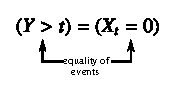
\includegraphics{figure/fig2.eps}}
\smallskip

But we have seen
\begin{align*}
P(X_{t}=0) &= e^{-\lambda t}\text{~~ so necessarily}\\[3pt]
P(Y>t) &= e^{-\lambda t}
\end{align*}
\end{proof}
\end{frame}

\begin{frame}
Now what about the analogue of the negative binomial = the waiting time for the $n$-th girl.

\myheading{The $r$-Erlang Distribution}

Let $Y_{r}=$ the waiting until the $r$-th animal is caught.

\begin{nonumtheorem}
\begin{itemize}
\item[(i)] The $cdf$ $F_{r}$ of $Y_{r}$ is given by
$$
F_{r}(t)=
\left\{
\begin{array}{l}
1-(1+\lambda+\frac{(\lambda t)^{2}}{2!}+\cdots+\dfrac{(\lambda t)^{r-1}}{(r-1)!},e^{-\lambda t},t>0\\
0,\text{~ otherwise}
\end{array}
\right.
$$

\item[(ii)] Differentiating (this is tricky) $F_{r}(t)$ to get the $pdf$ $f_{r}(t)$ we get
$$
f_{r}(t)=
\left\{
\begin{array}{ll}
\dfrac{\lambda^{r}t^{r-1}}{(r-1)!} e^{-\lambda t}, & t>0\\
0, & \text{otherwise}
\end{array}
\right.
$$
\end{itemize}
\end{nonumtheorem}

\begin{nonumremark}
This distribution is called the $r$-Erlang distribution.
\end{nonumremark}
\end{frame}

\begin{frame}
\begin{nonumproof}
We use the same trick as before
$$
P(Y_{r}>t)=P(X_{t}\leq r-1)
$$
The waiting time for the $r$-th animal to arrive in the trap is $>t\Leftrightarrow$ at time $t$

there are $\leq r-1$ animals in the trap.

Since $X_{t}\sim P(\lambda t)$ we have
\begin{align*}
P(X_{t}\leq r-1) &= e^{-\lambda t} +e^{-\lambda t}\lambda t+e^{-\lambda t}\dfrac{(\lambda t)^{2}}{2!}\\[3pt]
                &\quad +\cdots+e^{-\lambda t}\dfrac{(\lambda t)^{r-1}}{(r-1)!}
\end{align*}
\end{nonumproof}
\end{frame}

\begin{frame}
\begin{nonumproof}[Cont.]
Now we have to do some hard computation.
$$
P(X_{t}\leq r-1)=e^{-\lambda t}\left(1+\lambda t+\cdots+\dfrac{(\lambda t)^{r-1}}{(r-1)!}\right)
$$
So
\begin{align*}
F_{r}(t) &= P(Y_{r}\leq t)=1-P(Y_{r}>t)\\
        &= 1-e^{-\lambda t}\left(1+\lambda t+\cdots + \dfrac{(\lambda t)^{r-1}}{(r-1)!}\right)
\end{align*}
But\quad $f_{r}(t)=\dfrac{dF_{r}}{dt}(t)$

So we have to differentiate the expression on the right-hand side
$$
\text{Of course\quad } \dfrac{d}{dt}(1)=0
$$
\end{nonumproof}
\end{frame}

\begin{frame}
\begin{proof}[Proof (Cont.)]
\myheading{A hard derivative computation}
\begin{align*}
f_{r}(t) &=-\dfrac{-d}{dt}(e^{-\lambda t})\left(1+\lambda t+\dfrac{(\lambda t)^{2}}{2!}+\cdots+\dfrac{(\lambda t)^{r-2}}{(r-2!)}+\dfrac{(\lambda t)^{r-?}}{(r-1)!}\right)\\
&\quad -e^{-\lambda t}\dfrac{d}{dt}\left(1+\lambda t+\dfrac{(\lambda t)^{2}}{1!}+\cdots+\dfrac{(\lambda t)^{r-1}}{(r-1)?}\right)\\
&= \lambda e^{-\lambda t}\left(1+\lambda t + \dfrac{(\lambda t)^{2}}{2!}+\cdots+\dfrac{(\lambda t)^{r-2}}{(r-2)!}+\dfrac{(\lambda t)^{r-1}}{(r-1)!}\right)\\[3pt]
&\quad -e^{-\lambda t}\left(\lambda +\lambda^{2} t + \dfrac{\lambda^{3}t^{2}}{2!}+\cdots+\dfrac{\lambda^{r-1}t^{r-2}}{(r-2)!}\right)\\
&=e^{-\lambda t}\left(\cancel{\lambda}+\cancel{\lambda^{2}}++\cancel{\dfrac{\lambda^{3}t^{2}}{2!}}+\cdots+\cancel{\dfrac{\lambda^{r-1}t^{r-2}}{(r-2)!}}+\dfrac{\lambda^{r}t^{r-1}}{(r-1)!}\right)\\[3pt]
&\hspace{1.35cm} \updownarrow\quad\, \updownarrow\qquad\quad \updownarrow\hspace{2.2cm} \updownarrow\\
&\quad -e^{-\lambda t}\left(\cancel{\lambda}+\cancel{\lambda^{2}}++\cancel{\dfrac{\lambda^{2}t^{2}}{2!}}+\cdots+\cancel{\dfrac{\lambda^{r-1}t^{r-2}}{(r-2)!}}\right)\\
&= \dfrac{\lambda^{r}t^{r-1}}{(r-1)!}e^{-\lambda t}
\end{align*}
\end{proof}
\end{frame}

\begin{frame}
\myheading{Lifetimes and Failure Times for Components and Systems}

\smallskip
\centerline{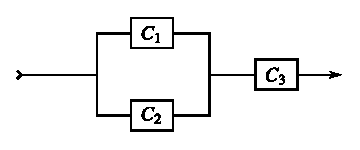
\includegraphics{figure/fig3.eps}}
\smallskip

Suppose each of the components has a lifetime that is exponentially distributed with parameter $\lambda$ (see below for a more precise statement). 

Assume the components are independent. How is the system lifetime distributed?
\end{frame}

\begin{frame}
\begin{nonumsolution}
Define random variables $X_{1},X_{2},X_{3}$ by
$$
(X_{i}=t)=(C_{i}\text{~ fails at time } t), i=1,2,3
$$
Then $X_{i}$ is exponentially distributed with parameter $\lambda$ so
\begin{align*}
& P(X_{i}\leq t)=1-e^{-\lambda t},i=1,2,3\\
& P(X_{i}>t)=e^{-\lambda}, i=1,2,3.
\end{align*}
Define $Y$ by
$$
(Y=t)=(\text{system fails at time $t$})
$$
\end{nonumsolution}
\end{frame}

\begin{frame}
\begin{nonumsolution}[Cont.]
The key step (using the geometry of the system)

Lump $C_{1}$ and $C_{2}$ into a single component $A$ and let $W$ be the corresponding random variable so
$$
(W=t)=(A\text{~ fails at time $t$})
$$

\centerline{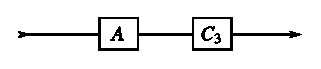
\includegraphics{figure/fig4.eps}}
$$
(Y>t)=(W>t)\cap (X_{3}>t)
$$
(the system is working at time $t$ $\Leftrightarrow$ \underline{both} $A$ and $C_{3}$ are working at time $t$)
\end{nonumsolution}
\end{frame}

\begin{frame}
\myheading{The Golden Rule}

Try to get $\cap$ instead of $\cup$ - that's why I choose $(Y>t)$ on the left.

Hence
\begin{align*}
P(Y>t) &= P((W>t)\cap (X_{3}>t))\\
       &\text{by independence}\\
       &=P(W>t)\cdot P(X_{3}>t)\tag{$\sharp$}\label{eq-sharp}
\end{align*}
Why are $(W>t)$ and $(X_{3}>t)$ independent?

\begin{answer}
Suppose $C_{1}$, $C_{2},\ldots C_{n}$ are independent components. Suppose 

$A$ = a subcollection of the $C_{i}$'s.

$B$ = another subcollection of the $C_{i}$'s.
\end{answer}
\end{frame}

\begin{frame}
\begin{answer}[Cont.]
Then $A$ and $B$ are independent $\Leftrightarrow$ they have no common component.

So now we need
$$
P(W>t)\text{~ where~ } W \text{~ is}
$$
\centerline{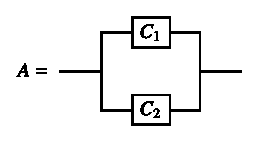
\includegraphics{figure/fig5.eps}}
\smallskip

I should switch to $P(W\leq t)$ to get intersections but I won't to show you why unions give extra terms.
\end{answer}
\end{frame}

\begin{frame}
$$
(W>t)=(X_{1}>t)\cup (X_{2}>t)
$$
($A$ is working at time $t$ $\Leftrightarrow$ either $C_{1}$ is or $C_{2}$ is)

So
\smallskip
\centerline{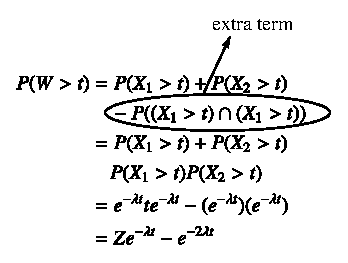
\includegraphics{figure/fig6.eps}}
\end{frame}

\begin{frame}
Now from \eqref{eq-sharp}
\begin{align*}
P(Y>t) &= P(W>t)P(X_{3}>t)\\
       &= (2e^{-\lambda t}-e^{-2\lambda t})e^{-\lambda t}\\
P(Y>t) &= 2e^{-2\lambda t}-e^{-3\lambda t}
\end{align*}
so the $cdf$ of $Y$ is given by
\begin{align*}
P(Y\leq t) &= 1-P(Y>t)\\
           &= 1-2e^{-2\lambda t}+e^{-3\lambda t}
\end{align*}
That's good enough.
\end{frame}
\end{document}


